\documentclass{scrartcl}
\usepackage[utf8]{inputenc}
\usepackage{amsmath,amssymb,amstext}
\usepackage{mathtools}
\usepackage{hyperref}
\usepackage{graphicx}

\graphicspath{ {images/} }
\usepackage[onehalfspacing]{setspace}

\begin{document}
	
	\title{Energy Online}
	\subtitle{}
	\author{J. Shah, M. Jordi, M. Stemmle, S. Oeschger, S. Zemljic}
	
	\pagenumbering{roman}
	\maketitle
	\newpage
	\tableofcontents
	\newpage
	
	\pagenumbering{arabic}
	
	\section{Introduction}
	
	\subsection{Context}
	
	\paragraph{}
	 The BIOTS program exists to push education for innovative new technologies into universities to help Switzerland o become one of the leading hubs in Blockchain and "internet of things" (IoT) space.\footnote{\url{http://biots.org/about/}}
	 
	\paragraph{}
	Since 2016, every year the BIOTS program offers three major verticals for the students to build their ideas and use-cases. In 2018, the focus was on sustainability issues, which are currently on the agenda of the UN or hot topics in industry. Challenges from the sponsors Elektrizitätswerk der Stadt Zürich (EWZ), UBS Group AG (UBS), the European founded project FuturICT 2.0 (\url{https://futurict2.eu}) across the following verticals were presented and solved in the program:
	
	\begin{figure} [h]
		\centering
		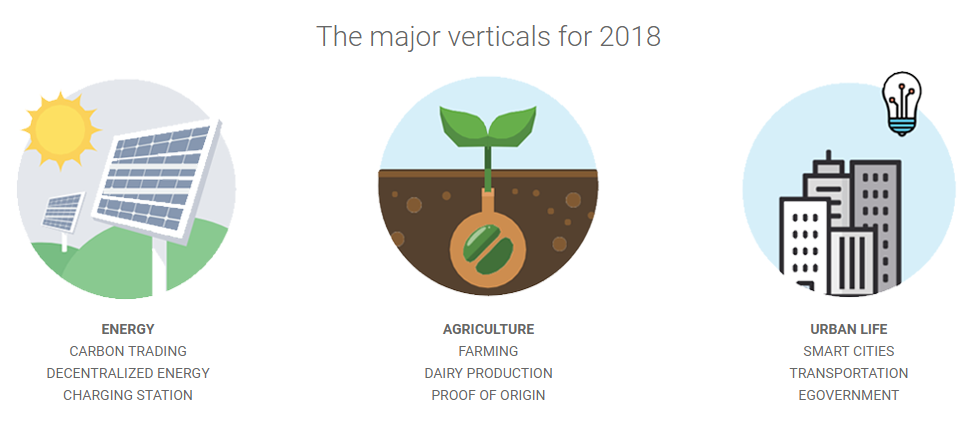
\includegraphics[width=100mm,scale=0.5]{01_introduction_picture01.PNG}
		\caption{Major verticals of BIOTS 2018, \url{http://biots.org/the-biotsphere/}}
	\end{figure}

	\paragraph{}
	This report was created as a solution to the challenge 3 “virtual energy storage” from EWZ.
	
	\subsection{Background}
	
	\paragraph{}
	In a cantonal vote 2017 it has been decided, that EWZ needs to sell all its holding in the nuclear sites of Gösgen and Leibstadt until 2034. In addition, EWZ will not be allowed to obtain nuclear energy anymore as well.\footnote{\url{https://www.nzz.ch/zuerich/aktuell/abstimmungssonntag-zuerich-atomausstieg-zuerich-ld.130738}}
	
	\paragraph{}
	In 2016 32.8\% of the electricity in Switzerland is provided by nuclear power plants.\footnote{Schweizerische Elektrizitätsstatistik 2016, p. 5: \url{http://www.bfe.admin.ch/php/modules/publikationen/stream.php?extlang=de\&name=de_306571764.pdf}} To be able to cover those losses, massive investments into renewable energy are needed. Large power plants alone will not be enough to cover the demands, thus small-scale energy production, like private PV's will play a huge role.
	
	\paragraph{}
	Currently, the entry barriers for the installation of PV are high, battery storage for surplus energy is expensive and overall incentives are missing. For example, energy surplus from private power plants (mainly PV) can only be sold to local energy provider for a very low price of 8.50 Rp./kWh (high tariff) or 4.45 Rp./kWh (low tariff).\footnote{\url{https://www.ewz.ch/content/dam/ewz/services/dokumentencenter/energie-produzieren/dokumente/verguetung-stromruecklieferung-zh-2016-18.pdf)}} To encourage the installation of PV, promotional money is lacking.\footnote{\url{https://www.srf.ch/news/schweiz/abstellgleis-solarenergie-wer-foerdergelder-will-muss-jahre-warten}}

	\paragraph{}
	To reach the goal of 0\% nuclear energy it is important to make private power plants more lucrative. Therefore, the challenge 3 of EWZ deals with the topic "Virtual Energy Storage". Virtual Energy Storage allows private household to store their surplus energy virtually and withdraw it later when needed.
	
	\paragraph{}
	This concept has been already adapted   Companies like eOn or SENEC already offer services like this to their customers:
	
	\paragraph{}
	eOn (\url{https://www.eon-solar.de/eon-solarcloud})
	
	\begin{itemize}
		\item Service Name:	E.ON SolarCloud
		\item Value Proposition: Genießen Sie jetzt Ihre Sonnenenergie 365 Tage, und Nächte
		\item Value Chain: E.ON to End customer
		\item Revenue Model: Monthly Fee
		\item Customer Segment: Private Households with PV installations
	\end{itemize}
	
	\paragraph{}
	Senec-ies (\url{https://www.senec-ies.com/tarife-services/senec-cloud/})
	
	\begin{itemize}
		\item Service Name: SECNEC.CLOUD 2.0
		\item Value Proposition: Strom im Sommer einfrieren und im Winter wieder auftauen.
		\item Value Chain: SENEC to End customer
		\item Revenue Model: Monthly Fee
		\item Customer Segment:	Private Households with PV installations
	\end{itemize}

	\paragraph{}
	Due to the companies and customers are trusted parties in those two services offerings, the necessity of the blockchain technology is not given. According to Karl Wüst and Arthur Gervaisy, “Blockchain is being praised as a technological innovation which allows to revolutionize how society trades and interacts. This reputation is in particular attributable to its properties of allowing mutually mistrusting entities to exchange financial value and interact without relying on a trusted third party. A blockchain moreover provides an integrity protected data storage and allows to provide process transparency.”\footnote{“Do you need a Blockchain?”, Karl Wüst, Arthur Gervaisy, \url{https://eprint.iacr.org/2017/375.pdf}}
	
	\subsection{Problem Statement}
	
	\begin{figure} [h!]
		\centering
		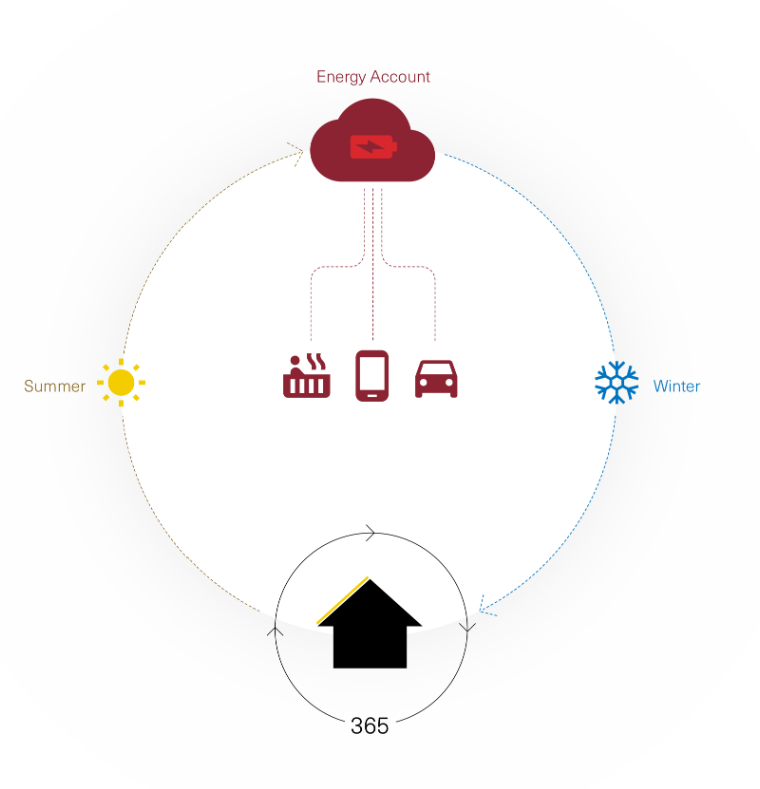
\includegraphics[width=80mm,scale=0.5]{01_introduction_picture02.PNG}
		\caption{EWZ Challenge 3 - "Virtual Energy Storage", Source: \url{EWZ (2018). BIOTS2018 ewz challenges. [Powerpoint slides]. Retrieved from https://slack-files.com/T8XEZNB4P-F98H4NZFD-8f3ddbc3b4}}
	\end{figure}
	
	The problem statement given by the EWZ Challenge 3 “Virtual Energy Storage” is: "How might the blockchain technology help to develop a reliable and highly efficient virtual energy solution that gives anyone the possibility to produce, store and use his/her own energy anywhere and anytime?"\footnote{“EWZ (2018). BIOTS2018 ewz challenges. [Powerpoint slides]. Retrieved from \url{https://slack-files.com/T8XEZNB4P-F98H4NZFD-8f3ddbc3b4}”}
	
	\section{Today’s blockchain application in the electricity sector}
    
    \paragraph{}
    The term ‘Blockchain technology’ refers to distributed databases with consensus algorithms that contain cryptographically concatenated data structure on which applications are built. The disruptive element is the ability to maintain a database that is shared in which everyone has access to all of the data however no one party has the ability to take over total control or perform modifications.\footnote{Mattila, Juri, Seppälä, Timo, Naucler, Catarina, Stahl, Riitta, Tikkanen, Marianne, Badenlid, Alexandra \& Seppälä, Jane (11.10.2016). “Industrial Blockchain Platforms: An Exercise in Use Case Development in the Energy Industry”. ETLA Working Papers No 43. \url{http://pub.etla.fi/ETLA-Working-Papers-43.pdf}} Blockchain is essential when trust needs to be established without a central authority and value needs to be transferred between stakeholders. This distributed ledger technology deployed using ‘smart contracts’ has immense applications\footnote{Ølnes, S., Ubacht, J., \& Janssen, M. (2017). Blockchain in government: Benefits and implications of distributed ledger technology for information sharing. Government Information Quarterly, 34(3), 355–364.}\footnote{Walport, M. (2015). Distributed ledger technology: Beyond block chain. Government Office for Science, 1–88. Retrieved from \url{https://www.gov.uk/government/publications/distributed-ledger-technology-blackett-review}}\footnote{Swan, M. (2015). Blueprint for a new economy. O’Reilly Media, Inc. \url{https://doi.org/10.1017/CBO9781107415324.004}} especially in the energy sector involving smart grids.\footnote{Pop, C., Cioara, T., Antal, M., Anghel, I., Salomie, I., \& Bertoncini, M. (2018). Blockchain based decentralized management of demand response programs in smart energy grids. Sensors (Switzerland), 18(1), 162. \url{https://doi.org/10.3390/s18010162}}
    
    \paragraph{}
    We find that for EWZ, being the central authority, which establishes trust, having a blockchain is not essential for storing virtual energy from users that produce sustainable energy. EWZ should use a business model as the one used by eon\footnote{Eon: \url{https://www.eon-solar.de/eon-solarcloud}} to store solar/wind energy produced by charging the producers a fixed rate and sell the energy for a profit. However, we see that blockchain has a potential application in the heavily regulated power industry (e.g. certificates) when both utilities and consumers will produce and sell electricity. Blockchain could in that case offer a reliable, low-cost way for financial or operational transactions to be recorded and validated across a distributed network with no central point of authority.
    
    \paragraph{}
    Since sustainability has been ranking higher than ever before on the global agenda of companies and governments alike, there have been considerable research and development on renewable sources of energy. The energy system will become more decentralized and versatile wind turbine parks and household solar panels are a growing trend in the generation of electricity and primary energy in general. This transition towards renewable energy means that energy production will become unpredictable and intermittent due to weather dependency associated with solar and wind energy, and hence requires long/short term demand-supply balancing.
    
    \paragraph{}
    The idea is that by creating a distributed marketplace powered by employing a blockchain consensus Blockchain technology could offer a way to circumvent this problem by providing a neutral ground where all the parties can operate on a shared platform, on completely equal footing. Instead of the platform provider like EWZ, BKW being the dominant player to the power of whom all others must submit, blockchain technology could enable all the participants to produce a platform together in a distributed manner, without having to trust each other in almost any capacity. Some earlier use case concepts have been drafted which focus on allocating distributed renewable energy resources between neighboring households using blockchain technology.\footnote{Harvard Business review: \newline
    \url{https://hbr.org/2017/03/how-utilities-are-using-blockchain-to-modernize-the-grid}} For example, in New York state, neighbors are testing their ability to sell solar energy to one another using blockchain technology (Brooklyn-microgrid\footnote{Brooklyn Microgrid: \url{http://www.power-technology.com/features/featurethe-brooklyn-microgrid-blockchain-enabled-community-power-5783564/}}). In Austria, the country’s largest utility conglomerate, Wien Energie\footnote{Wien Energie: \url{https://www.wienenergie.at/eportal3/}}, is taking part in a blockchain trial focused on energy trading with two other utilities. Meanwhile in Germany, the power company Innogy\footnote{Innogy: \url{https://iam.innogy.com//en/ueber-innogy}} is running a pilot to see if blockchain technology can authenticate and manage the billing process for autonomous electric-vehicle charging stations. Another example is PriWatt\footnote{Aitzhan, Nurzhan Zhumabekuly, and Davor Svetinovic. "Security and privacy in decentralized energy trading through multi-signatures, blockchain and anonymous messaging streams." IEEE Transactions on Dependable and Secure Computing (2016).}, which is a token-based energy trading system that allows to trade energy in a peer-to-peer network without a central price signal. The prosumer uses photo-voltaic panels harvests solar energy and makes profit by selling the generated energy surplus to the other smartgrid consumers. In a conventional power grid, energy prices are determined by a central authority like EWZ, BKW. In a smartgrid, agents are allowed to negotiate energy prices [5], hence creating a dynamic market of energy trade. Such a market-based energy trade decreases dependency of agents on a central energy provider, as energy supply and demand are matched directly between individual agents, resulting in a more decentralized and competitive environment. PriWatt satisfies this requirement and enables peers to anonymously negotiate energy price and securely perform trading transaction.
    
    \paragraph{}
    In our opinion although we might think that blockchain may at first appear to be a form of technological disruption that the power industry should avoid, it could prove to be the solution that is required to keep up with evolving demand for electricity. Established utilities like EWZ are best placed to evaluate and make strategic bets on blockchain technology’s potential applications. If EWZ can seize the moment, they may turn out to be the true disruptors, and usher in a new era of decentralized power.
	
	\section{Conceptual Design}
	
	\subsection{Overview}

    \paragraph{}
    Our approach to the EWZ Challenge 3 “Virtual Energy Storage” is to create a Decentralized Autonomous Organization (DAO). 
    
    \paragraph{}
    The DAO is not a potential future business model applicable for EWZ but demonstrates how the blockchain is in position to change the energy sector and illustrates the disruptive power due to the emerging areas of blockchain applications. However, our approach provides a "Virtual Energy Storage" of the participants of the DAO. In addition, we further address with the DAO an alternative for owners of real estate to the modest of governmental incentives to become a producer of renewable energy. With implementing such or a similar alternative blockchain based approach, it could be a way out of a potential electricity shortage due to the governmental regulation regarding the end of the production of electricity from nuclear sources in Switzerland by 2034. In this respect, the following DAO can be described as a catalyst of renewable energy. 
    
    \paragraph{}
    In the real world exists initiatives such as Brooklyn Microgrid that enables residents of the Park Slope area of Brooklyn, NY to sell power generated from rooftop solar panels via a microgrid enabled by a blockchain ledger that records every transaction made with a local utility.\footnote{\url{www.brooklynmicrogrid.com}} The DAO brings such an initiative a step further.
    
    \paragraph{}
    The DAO's behaviour is completely controlled by smart contracts and it fulfils functions similar to the ones of an energy provider today:
   
	\begin{itemize}
		\item Energy Management: \newline
		The DAO makes sure that there is sufficient energy available for all the participants of the systems and enables all parties to trade energy freely by using the energy token.
		
		\item Trading at the energy market: \newline
		The DAO sells surplus energy and buys energy if there is a shortage in the network on the traditional energy market.
		
		\item Profit distribution: \newline
		The DAO uses profits realized by trading to subsidize others to install renewable energy production possibilities and participate in the system. This enlarges the current system and creates additional surplus.
	\end{itemize}

	\paragraph{}
	Within the DAO, energy is traded freely amongst all participants by using energy tokens. Energy tokens represent the right to obtain energy from a participant of the system.
    
    \begin{figure} [h]
    	\centering
    	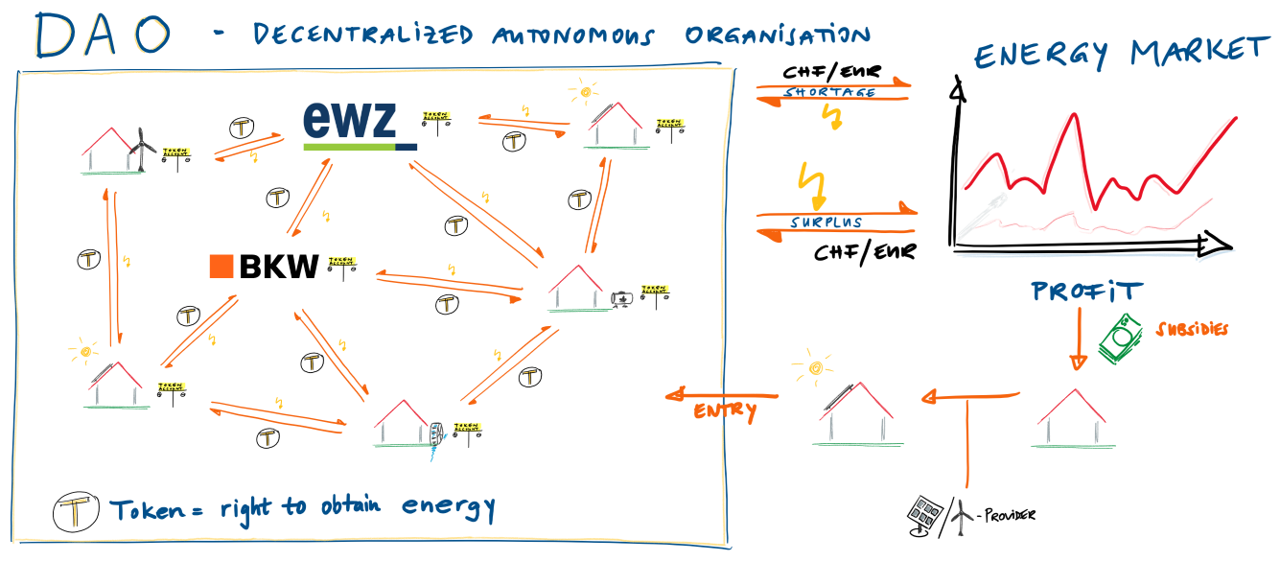
\includegraphics[width=145mm,scale=1]{03_conceptual_design_picture01.PNG}
    	\caption{Conceptual Design, Source: this report}
    \end{figure}
    
    \paragraph{}
    For other energy providers, the DAO can act as a virtual power plant which generates renewable energy. Due to the energy would be generated within Switzerland, the cost and lost of transportation would be lower compared to the purchase of energy abroad.
    
     \paragraph{}
     With this concept, the monopolistic Swiss energy market could be disrupted massively. Electricity could be freely traded peer to peer. The limitations through cantonal borders, would fall away, even trade across national borders could be possible at a later point. Current energy providers would take the role of a hardware provider, ensuring the maintenance of the energy grid and maybe the smart meters financed through fees for the usage of the infrastructure.
     
     \subsection{Decentralized Autonomous Organization DAO}
     
     \paragraph{}
     According to CHOHAN, a DAO, is an organization that is run through rules encoded as computer programs called “smart contracts”. A DAO's financial transaction record and programmed rules are maintained on a blockchain, which ostensibly increases transparency dramatically at the expense of security.\footnote{"The Decentralized Autonomous Organization and Governance Issues", Usman W. Chohan, December 4, 2017.}
     
     \paragraph{}
     A DAO is, according to SWAN, a potential progression to increasingly complex and automated smart contracts that become more like self-contained entity, conducting preprogrammed and eventually self-programmed operations linked to a blockchain.\footnote{“Blockchain – Blueprint for a New Economy”, Melanie Swan, 2015, O’Reilly Media, Inc.}
     
     \paragraph{}
     Vitalik Buterin, the visionary founder of Ethereum\footnote{\url{https://www.ethereum.org/}} sees three major categories where decentralized autonomous organizations may provide genuine value to society. Frist, when there are natural monopolies. Second, when there are services that violate government laws and regulations (e.g. the use of decentralized file-sharing networks for copyright infringement) and, finally, there are those cases where a decentralized network can simply maintain itself more efficiently and provides better services than any centralized alternative (i.e. peer-to-peer network).\footnote{"Bootstrapping a Decentralized Autonomous Corporation", Vitalik Buterin, September 24, 2013.} The DAO, according to Buterin, human managerial interactivity, provided the smart contracts were supported by a Turing complete platform.\footnote{Decentralized autonomous organization, \url{https://en.wikipedia.org/wiki/Decentralized_autonomous_organization}, retrieved February 25, 2018.} 
     
     \paragraph{}
     In essence a DAO is a system of hard coded rules that define which actions an organization will take, so the organization may run without managerial supervision or, if the platform provided sufficient rules and flexibility, completely autonomous. All rules upon which the company functions are enforced digitally.\footnote{Decentralized autonomous organization - What is a DAO company?, \url{https://medium.com/universablockchain/decentralized-autonomous-organization-what-is-a-dao-company-eb99e472f23e}, retrieved February 25, 2018.} "Other decisions are made by shareholders who control a certain amount of the tokens, or smart contracts, who can vote for decisions. Preprogrammed rules describe what can happen in the system. Certain rules are hard-coded into the company like the amount of dividend payouts or determining a certain event in the company. Other things like, determining which project will receive money is decided by letting all token holders cast their vote."\footnote{Decentralized autonomous organization - What is a DAO company?, \url{https://medium.com/universablockchain/decentralized-autonomous-organization-what-is-a-dao-company-eb99e472f23e}, retrieved February 25, 2018.}
     
     \paragraph{}
     There exist real world DAO projects such as for example, "Dash", "The DAO", "Digix.global", "Steemit". So far, DAOs can be found mainly in the FinTech sector, where they can benefit from a sophisticated organizational structure and the resulting rapid decision-making processes in a volatile and fast-moving market.
     
     \paragraph{}
     A DAO must be able to make decisions, be liquid and communicate with internal and external bodies. After all, money must get into the organization, employees and service providers must be remunerated and interaction with the rest of the world must be possible. As a result, several components are required which are essential for a DAO:\footnote{What is a DAO?, \url{https://blockchainhub.net/dao-decentralized-autonomous-organization}, retrieved February 25, 2018.}\footnote{Decentralized Autonomous Organization – Organisationen auf der Blockchain, Jonas Verhoelen, \url{https://blog.codecentric.de/2017/08/decentralized-autonomous-organization-blockchain}, retrieved February 25, 2018.}
    
    \begin{itemize}
    	\item Autonomy: \newline
    	Once deployed the entity is independent of its creators and cannot be influenced by outside forces. DAOs are open source, thus transparent and incorruptible. A DAO’s financial transaction record and program rules are maintained on a blockchain. This approach eliminates the need to involve a bilaterally accepted trusted third party in a financial transaction.
    	
    	\item Currency / Tokens: \newline
    	In order not to bind the organization to a central currency, the DAO's ecosystem should have its own currency, also known as "tokens". This is used for payment, external investments and finally the accumulation of wealth within the organization. As a result, the DAO is at least internally liquid. Of course, financial interactions with the outside world take place via a change point. An indirect point of contact with traditional centralized Fiat money such as the dollar or the Euro thus seems to be unavoidable so far.
    	
    	\item Contractors: \newline
    	Members of the organization can have an influence on the development of the organization and can also be involved in the implementation of the adopted proposals. However, a DAO cannot build a product, write code or develop hardware. It needs a contractor or external service providers to accomplish its goals. Such Contractors get appointed via voting of token holders and payment can be made either in the own currency or by partial liquidation in Fiat currencies.
    	
    	\item Proposals and Voting: \newline
    	Decisions about the future of the organization must be made before it can develop further. Proposals are the primary way for making decisions in a DAO. Proposals may be raised by any member of the organization (or a specific role in the organization). To avoid people overloading the network with proposals, a DAO could require a monetary deposit to prevent people from spamming the network. After submitting a proposal, voting takes place. 
    	
    	\item Consensus: \newline
    	In order to withdraw or move funds from a DAO, a majority of its stakeholders (this percentage could be specified in the code of the DAO) must agree on the decision. Even if bugs are found in the code, they could not be corrected until a voting procedure has taken place and the majority of voters agreed on it, which could leave known security holes open to exploitation.
    	
    	\item Transparency: \newline
    	All processes and mechanisms must be fully transparent to members of the organization. Everyone should be able to participate and work together. By recording all aspects and processes on the blockchain, this is also possible and manipulation is made theoretically impossible.
    \end{itemize}

	\begin{figure} [h]
		\centering
		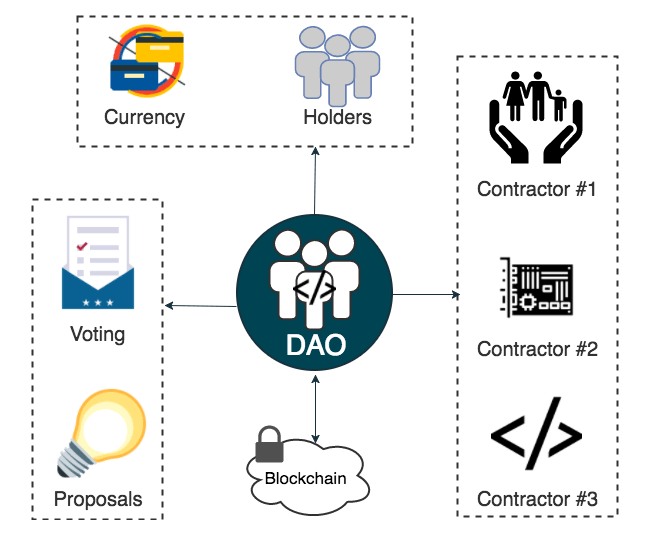
\includegraphics[width=100mm,scale=0.5]{DAO's_components_Jonas_Verhoelen.png}
		\caption{A DAO's components, source: Jonas Verhoelen, https://blog.codecentric.de/2017/08/decentralized-autonomous-organization-blockchain/}
	\end{figure}

	\subsection{Characteristics and functionalities of our proposed DAO}
	
	\subsubsection{Energy Management}
	
	\begin{figure} [h]
		\centering
		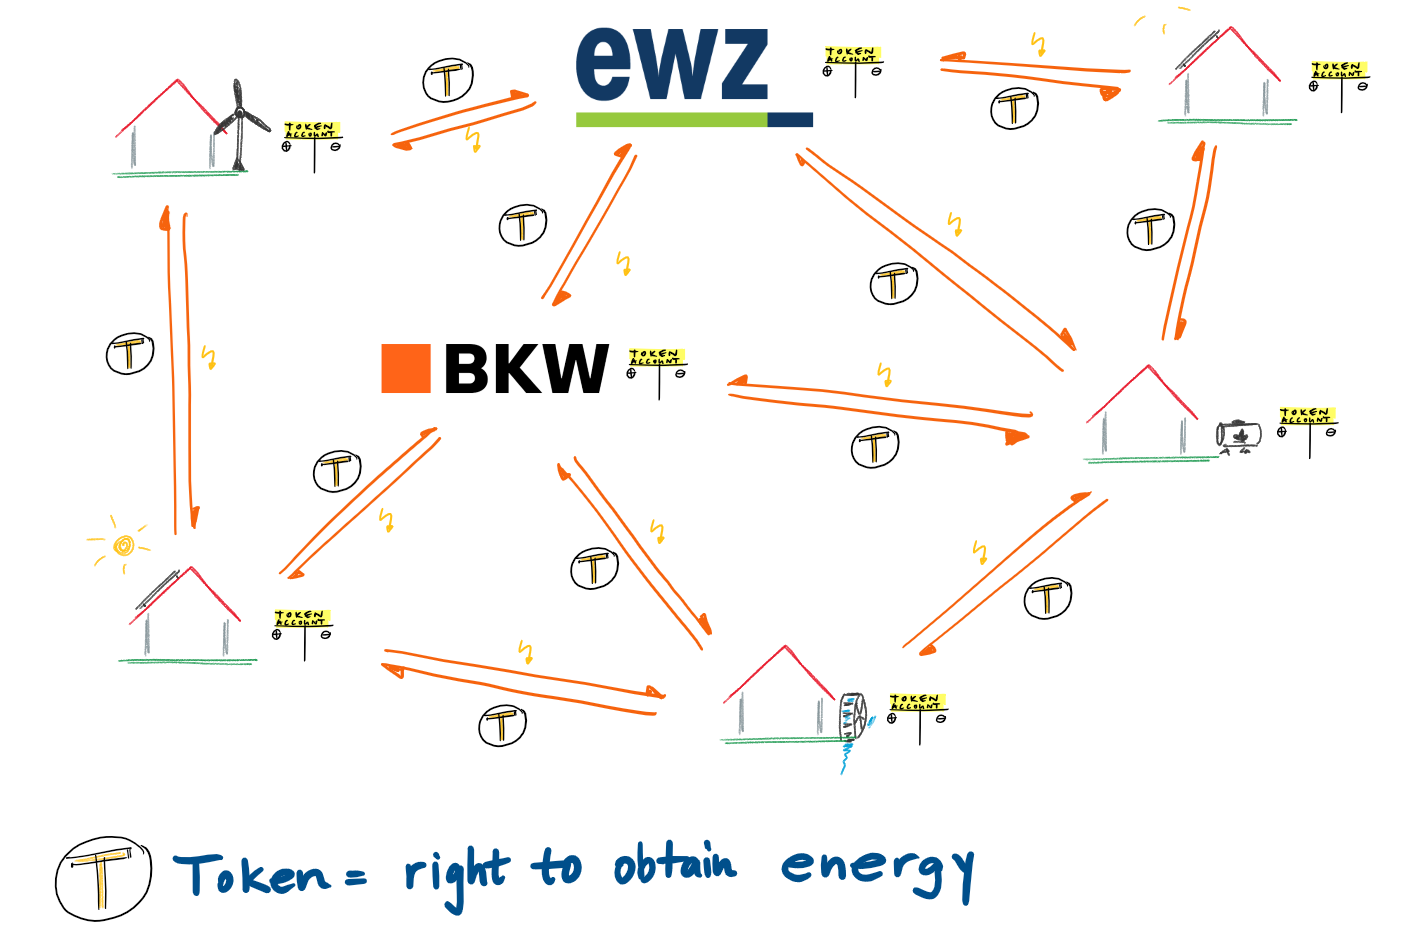
\includegraphics[width=100mm,scale=0.5]{section_3_3_1.png}
	\end{figure}
	
	\paragraph{}
	As a precondition to be part of the system, every participant in the DAO is a user or a provider of renewable energy via wind, solar or hydropower. Such a participant is called "prosumer". The different participants such as real estate owners with solar panels or power suppliers such as EWZ with access to renewable energy provide electricity that flows into the system's grid. Electricity consumers are the producing or other households or companies of the area of the DAO. The DAO interconnects prosumers and/or provide a direct link between energy suppliers and energy consumers.
	
	\paragraph{}
	All electricity produced and consumed by a household is tracked by a smart electric meter that is connected to a virtual energy balance sheet.  A Household may use its electricity produced by its own energy production facility or feed the power to the system, if it has a surplus. The household receives Tokens for a certain amount of electricity produced and it gives Tokens, if it does not produce enough own electricity, when it receives power of another energy provider's surplus. In case a household has consumed all its Tokens (e.g. uses more energy during night then it can produce during the day) and the virtual balance sheet shows a negative balance, it may buy energy Tokens from the DAO or a system participant with Fiat currency.
	
	\paragraph{}
	If the DAO's energy system provides an energy surplus the surplus may be traded on the energy market or in case of the system's energy shortage additional energy is purchased.
	
	\subsubsection{Trading at the energy market}
	
	\begin{figure} [h]
		\centering
		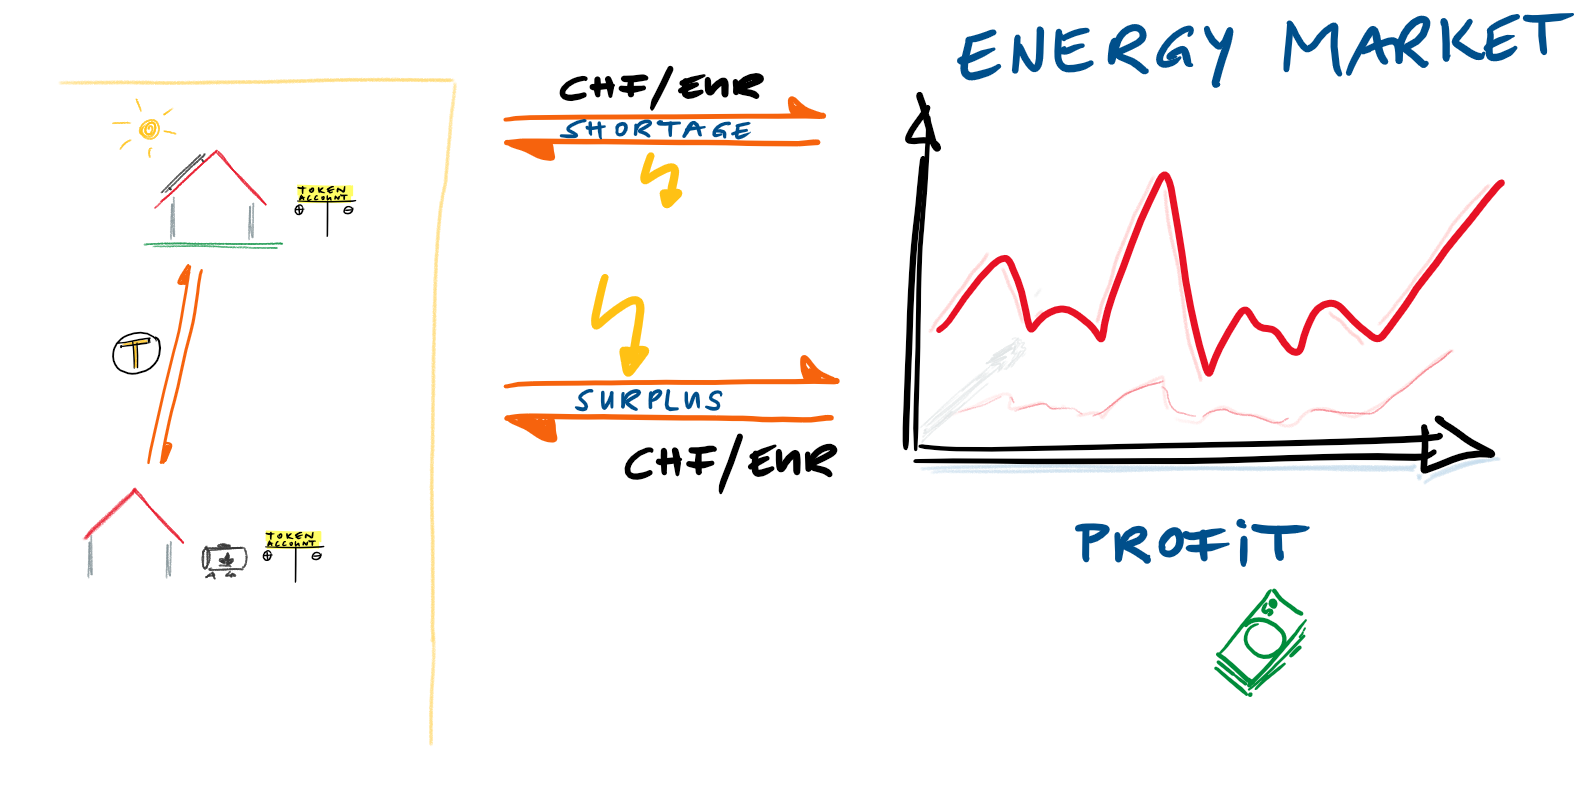
\includegraphics[width=100mm,scale=0.5]{section_3_3_2.png}
	\end{figure}
	
	\paragraph{}
	The DAO's financial transaction, how energy surplus is traded and how energy shortfall is covered, is predefined in programmed rules and defined by smart contracts. This approach eliminates the need to involve a bilaterally accepted trusted third party in the financial transaction. In addition, the DAO acts fully rational and is not biased by external conditions.
	
	\paragraph{}
	If the DAO may sell its electricity surplus, e.g. when during sunny daytime the member's solar PV panels produce an electricity excess, the DAO may achieve high prices, since during daytime also electricity prices are highest.
	
	\paragraph{}
	Because the electricity exchange will not accept the tokens of the system, all financial transactions by or with the DAO are made with Fiat money (e.g. CHF, EUR).
	
	\subsubsection{Profit distribution}
	
	\begin{figure} [h]
		\centering
		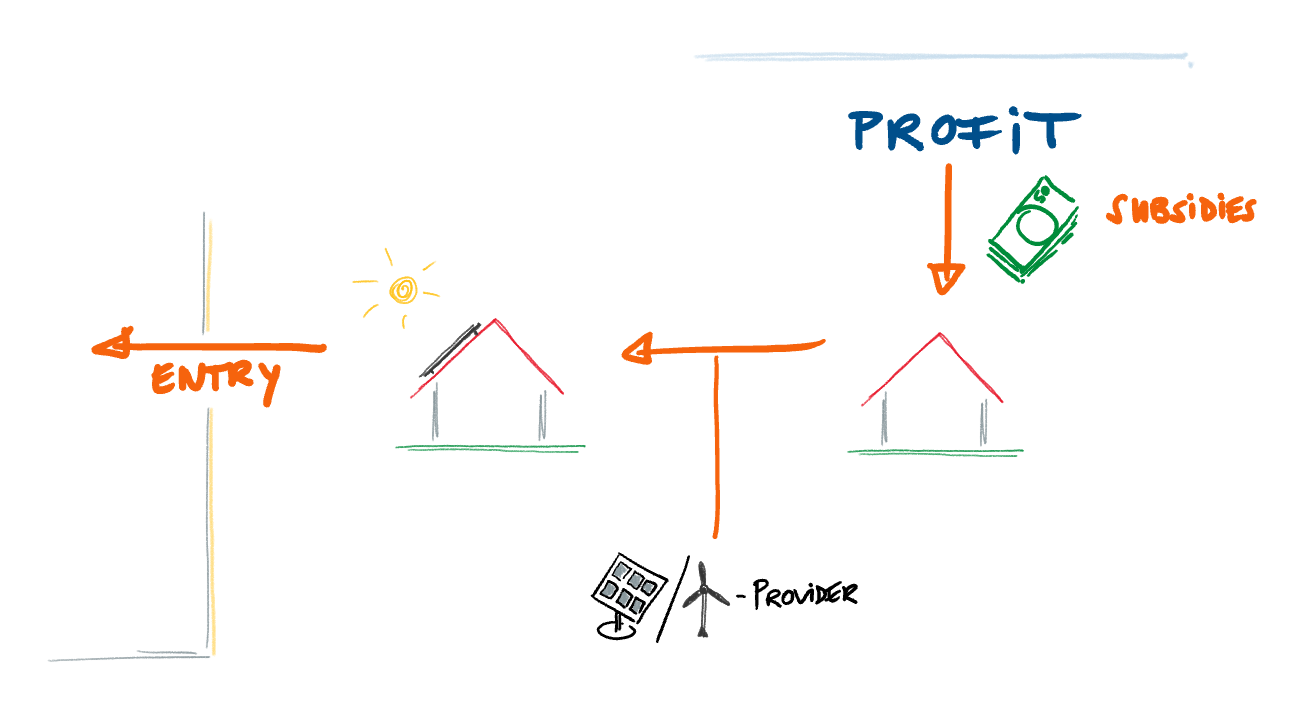
\includegraphics[width=100mm,scale=0.5]{section_3_3_3.png}
	\end{figure}
	
	\paragraph{}
	If the system's energy surplus is bigger than the energy bought during an electricity shortage and the DAO's smart contracts are well established so that it sells the green energy to the highest prices possible, the DAO's trading activity will produce a profit. With the profit made from trading, the DAO pays subsidies to more households, companies or other renewable energy projects to build renewable power plants and thus enlarging its network.
	
	\paragraph{}
	All processes and mechanisms must be fully transparent to members of the organization. According to the DAO's governance structure and the underlying smart contracts, the DAO's members or specific roles in the organization may vote how the profit is spent. Also other important developments of the DAO need to be voted about or created consensus among the members with voting power. The members of the organization may have an influence in e.g. what share of the profit is hold reserved for electricity shortage or which share of the profit should be allocated in the form of subsidies to which type of projects (e. g. wind, water, solar energy, etc.) to make the network and its independence even stronger. A balanced network of energy suppliers (e. g. solar, water and wind power plants) can bridge the shortfall of electricity at night or in winter, which must be taken into account in investment projects in order to be as autonomous as possible and generate maximum profit.
	
	\subsubsection{Energy Token}
	
	\paragraph{}
	The DAO's ecosystem issues its own currency in form of Tokens. A Token holder has the right to obtain specified energy from the system in return of a specified number of Tokens or the receives Tokens in exchange of providing energy to the grid. Depending on the day or night tariff, the "electricity price" paid in tokens also changes within the DAO network. 
	
	\paragraph{}
	Therefore, insofar as an electricity producer has the opportunity to regulate the amount of electricity that can be supplied to the system (e. g. electricity production by hydroelectric power plants at peak times or in times of little sunshine), an incentive arises to build such adaptive power plants and/or produce electricity, when prices are highest and the most Tokens can be generated.
	
	\subsection{Initialization of the Concept}
	
	\paragraph{}
	At the beginning, there will be an "Initial Coin Offering" (ICO), to get the initial funds for the DAO and to distribute the Tokens. This process would give the DAO its starting capital to start investing in renewable energy, and then trade on the energy stock market. A major part of the Tokens will be sold to investors and given to energy producers. A smaller part could be distributed for example to core developers or held back as reserves. Only producers of renewable energy are allowed to participate in the ICO.
	
	\subsection{Disruption Potential}
	
	\paragraph{}
	The underlying transaction model of the blockchain technology lead to a decentralized system, where energy producer and end customers or energy companies can directly start to trade. Third party intermediaries are no longer needed, if the transaction may be carried out peer-to-peer, regardless of territorial borders such as cantonal or municipal boundaries and (unless regulated) also in circumvention of a sovereign monopoly. This ensures that existing power generation capacity is utilized optimally, whilst energy is made available at the best price. And since the system's tasks are carried out automatically through smart contracts, this cuts costs and speeds up processes. The role of prosumers is strengthened considerably under such a model.\footnote{“Blockchain – an opportunity for energy producers and consumers?”, PwC, 2015.}
	
	\paragraph{}
	Due to the rational acting and maximal efficiency the DAO acts as a very efficient self-growing system. In addition, based on the smart electric meter and the virtual energy balance sheet of every prosumer and the prosumers ability to consume the positive balance of the green electricity produced during low performance of the own power facility, the DAO acts as a virtual power plant and as virtual energy storage.
	
	\paragraph{}
	EWZ and other power plant owner’s role in a Decentralized Autonomous Organization will change dramatically. EWZ will not be a monopolist in its territory, but a participant and provider of renewable energy. And since EWZ will be the provider and owner of the grid in its territory, EWZ will be paid via a certain fee or tax levy for the constant maintenance of the grid and the DAO's use of the grid. The payments could potentially be done with Tokens. The affiliate company of EWZ selling and installing PV facilities could act as one of many providers of all physical installations such as for example solar panels, network control systems, converters, and smart electric meters. In other words, in the present presentation of this DAO system, EWZ will only be a market participant, supplier and operator of the electricity grid. Power suppliers, such as EWZ, lose their monopolistic positions.
	
	\paragraph{}
	Therefore, the potential use cases of blockchain technology in the energy sector show a lot of promise and have the potential to radically change the energy market.
	
	\subsection{Evaluation}
	
	\paragraph{}
	Although the blockchain technology is very promising, first successful projects such as BrooklynMicrogrid are emerging and a DAO seems to work in theory, the implementation and introduction of a DAO in the Zurich or Swiss electricity market is associated with many hurdles. Furthermore, the experience with the blockchain technology is limited to only a few years.
	
	\paragraph{}
	As a result, virtual energy storage should be built up step-by-step in order to gain initial experience with its underlying business model and the new blockchain technology and to reduce internal and external resistance. With this experience, EWZ, together with other electricity producers and strategic partners, can develop a sophisticated concept and system around and for a DAO that integrates consumers, prosumers and electricity producers appropriately.
	
	\paragraph{}
	As a bootstrapping procedure, the following three phases could be established by EWZ:
	
	\begin{figure} [h!]
		\centering
		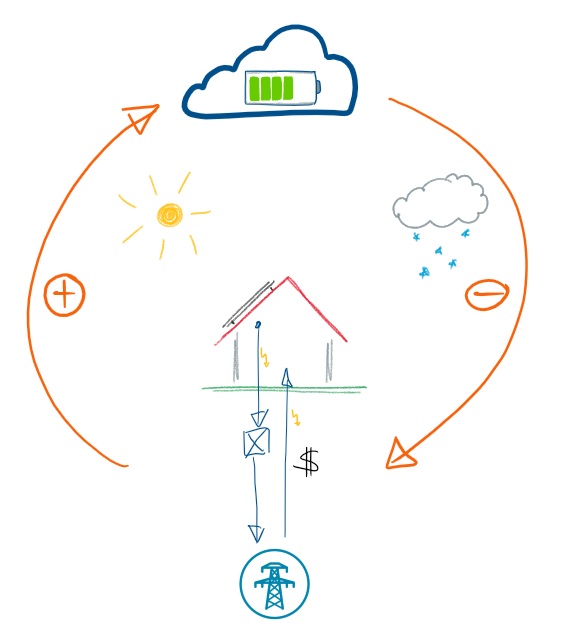
\includegraphics[width=60mm,scale=0.5]{Phase_1_EnergyCloud.PNG}
		\caption{Phase 1: Generating a business model of Virtual Energy Storage to create consumer’s interest}
	\end{figure}

	\begin{figure} [h!]
		\centering
		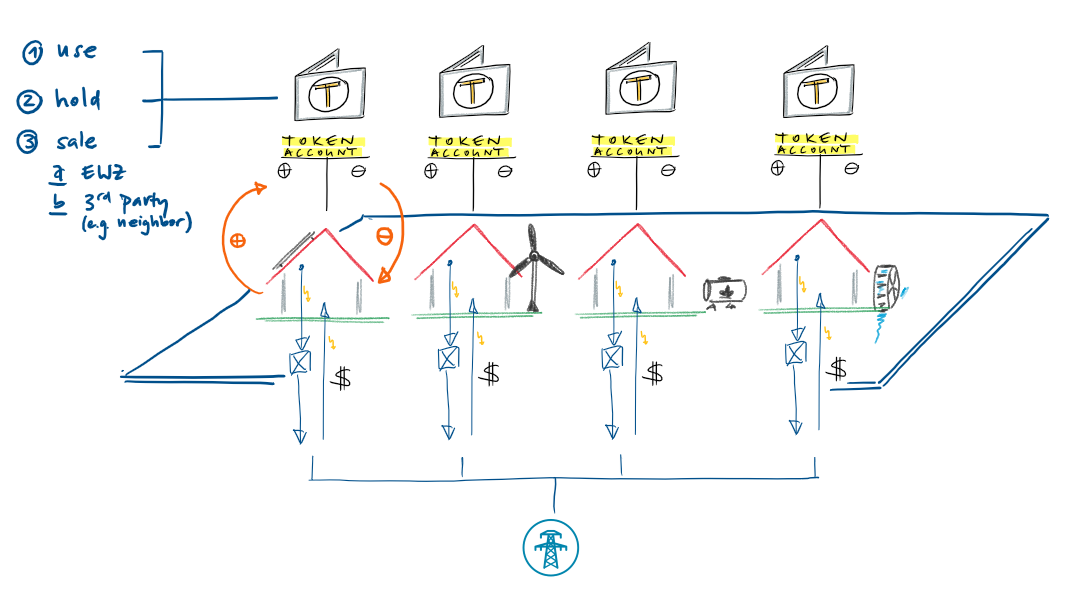
\includegraphics[width=100mm,scale=0.5]{Phase_2_EnergyCloud_Blockchain.PNG}
		\caption{Phase 2: Establish a blockchain based ecosystem for provider of renewable energy and accept issued Tokens as currency}
	\end{figure}
	
	\begin{figure} [h!]
		\centering
		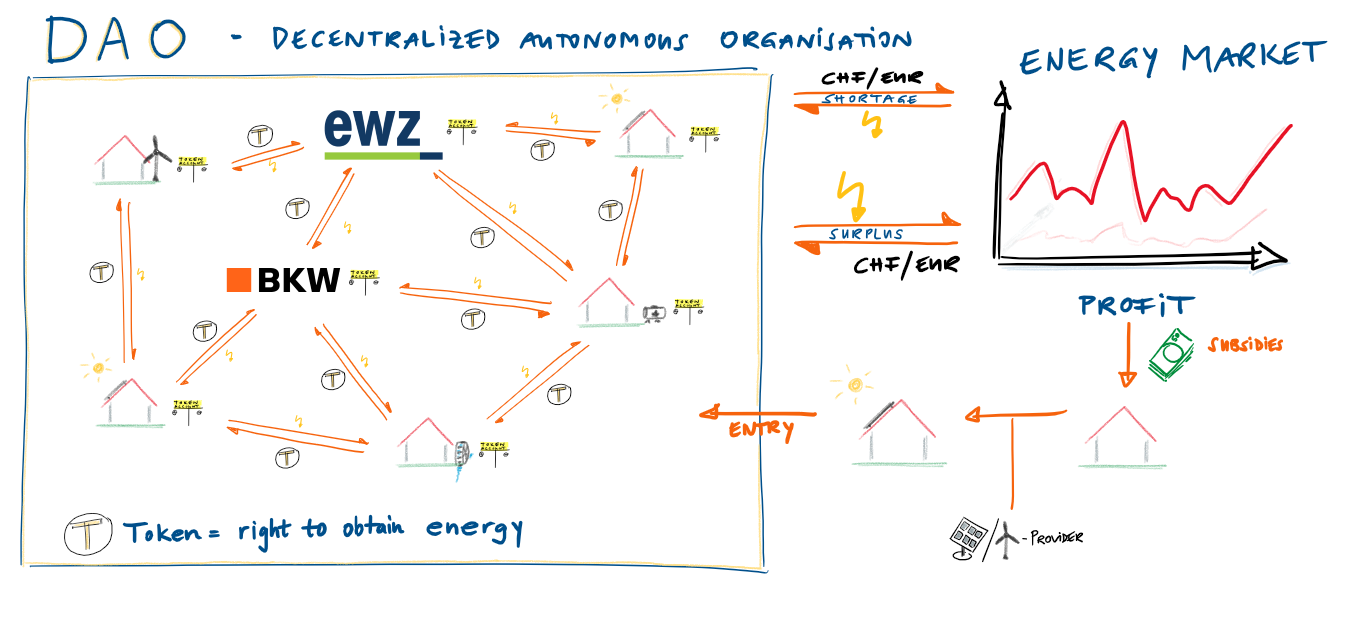
\includegraphics[width=100mm,scale=0.5]{Phase_3_DAO.PNG}
		\caption{Phase 3: Establish and implement a DAO}
	\end{figure}
	
	\subsection{Uncertainties, disadvantages and risks}
	
	\paragraph{}
	Blockchain as a technology and its applications and extensions in the form of a DAO require or overwhelm most people.  Not only because there is a need for in-depth technical understanding, but also because the disruptive upheaval is so significant that comparisons with what is known and the application of existing laws and regulations are almost impossible. Difficulties arise, for example, with the division into groups, what kind of a legal construct a DAO is, whether a "head office" of a DAO is possible at all due to the decentralized structure, how the system is taxed, whether and how transactions within the network have to be settled, what kind of liabilities exist for a physically non-existing construct owned by nobody, and so on.
	
	\paragraph{}
	Another controversial point is trust. Blockchains are supposed to build trust, so DAO's are organizations of trust, because every participant trusts that the system has been implemented fairly and is constantly improved. For example, because the system is implemented by smart contracts that are nothing more than distributed code, the entire organization is entrusted to one program. Programs continue to be developed by people who can make mistakes. Weak points in the respective blockchain software and the smart contracts executed on it are therefore a major risk. The DAO showed that a small mistake can bring down the house of cards. When it collapses, there is no saving authority or legal barrier that can help shareholders. All trust is in the code.\footnote{Decentralized Autonomous Organization - Organisationen auf der Blockchain, Jonas Verhoelen, \url{https://blog.codecentric.de/2017/08/decentralized-autonomous-organization-blockchain}, retrieved February 25, 2018.}
    
\section{Solution Design}
   
   \paragraph{}
   If we draw attention to the code behind our idea we can divide it into two parts: backend (solidity) and frontend (html, javascript, metamask). The purpose of the frontend is to give a simple but hopefully not less secure interface to the user so he can easily access the blockchain. The backend consists of the wallet contract (managing the tokens) and an example implementation of how some of the transfers could work. It is still not fully realistic because of the complexity of a more detailed model (and for purpose of presentation its not necessary). The focus of the following chapter is on the backend part because the frontend is quite simple. Frontend is just about letting metamask call some prepared functions of certain contracts on the blockchain, and about listening to events of the contracts (and showing these in a stylish and simple way to the user).
   
	\begin{figure} [h!]
		\centering
		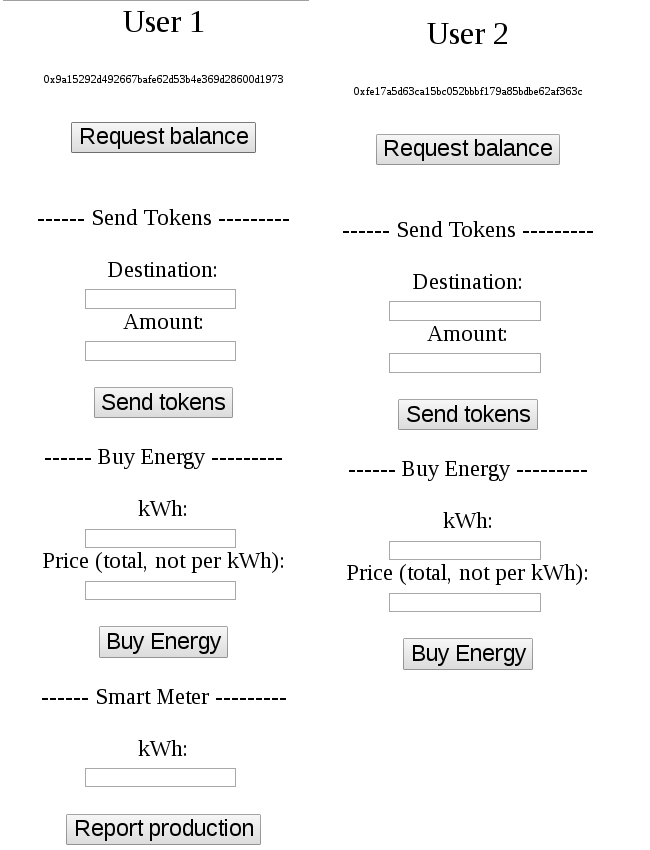
\includegraphics[width=100mm,scale=0.5]{section_4_users.PNG}
		\caption{Snapshots of the frontend implemented with html, javascript and MetaMask}
	\end{figure}
   
   \paragraph{}
   We will start with the abstract model of what we tried to build. Then the main part is about the implementation (in solidity) and it’s difficulties. The last part of the solution design will be about some problems with this implementation.
   
\subsection{Idea}
   
   \paragraph{}
   The main target of our implementation is, that it has to be secure. So we try to do it as simple as possible (then there are less sources of errors). Every user should be able to get a wallet where his tokens will be stored. Nobody else should have the right to take tokens out of that ‘bag’. But there should be some automation for the transactions (e.g when a user produces for or buys energy from the connecting network at his home).
	
	\paragraph{}
	To create the connection between the real world and the blockchain we use the concept of Smart-Meters. Any organization that got the trust of people in its environment could offer this service. Smart-Meters should measure the produced and consumed energy of users and report it to the blockchain, where Smart-Contracts between the user and the connecting network will transfer tokens dependent on the individual implementation of these Smart-Contracts.
	
	\subsection{Our Implementation}
	
	\paragraph{}
	The sources are available on GitHub (https://github.com/ETHBIOTS2018/EnergyOnline/Code/VersionReport/)
	
	\begin{figure} [h]
		\centering
		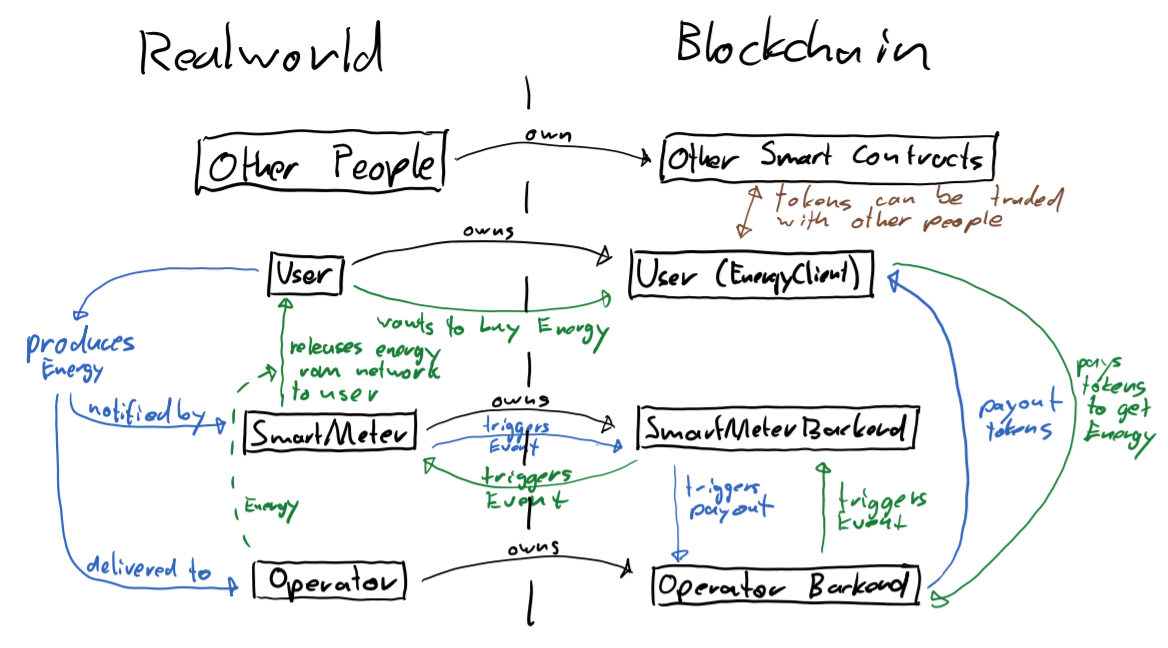
\includegraphics[width=150mm,scale=1.0]{section_4_flow_chart.PNG}
		\caption{The flow chart shows the 3 main actions that are possible in our implementation: User producing energy, User consuming energy and User trading tokens with other users.}
	\end{figure}
	
	\subsubsection{Wallet}
	
	\paragraph{}
	This contract is responsible for the ICO and it holds the balances of tokens. Therefore it should be really really simple. If there is a bug that can be exploited in this contract the whole concept could not work. We explain shortly the functions of this contract:
	
	\begin{itemize}
		\item When the wallet is constructed it will initialize the amount of coins on the market to 1e20. We did spend a lot research in how much this should be, so this could be changed. The owner is the creator of this contract. The owners address will get all the Ether that is given to this contract (the ether from the ICO).
		\item ‘transfer’ transfers an amount of tokens from the callers account to a destination account. It’s quite simple. It only works if there are enough tokens on the callers account and if the transaction happened it will fire an event, there is no need for overflow check because there are not enough tokens initialized to create an overflow. Frontend programs can listen on the fired events. In the Ethereum blockchain there is an extra section where fired events are listed, so everyone could check or listen to them.
		\item "buy Tokens" is the only payable function of this contract. It’s used for the ICO. For simplicity it just does a normal transfer of tokens from the wallets account to the callers account. The amount of tokens is equal to the amount of Wei (sub-currency of Ether) paid. Obviously the transaction gets cancelled if there are not enough tokens on the wallets account.
	\end{itemize}
		
	\subsubsection{Model Scenario}
	
	\paragraph{}
	The Wallet is the only part that will be the same for all transactions in different regions with different producers and consumers. The other three contracts just show a possible scenario how Smart-Contracts could do the transactions automatically.
	
	\paragraph{}
	Smart-Meter-Backend contains functions that can be called by the real (hardware) Smart-Meter that measures electricity in and outflow of a producer/consumer. In our implementation it has just one function that reports energy production to the network operator.
	
	\paragraph{}
	The Operator-Backend will need some more explanation. There are functions (that are called by the owner, as example EWZ) that set the price for electricity from this network and the reward for feeding energy into it. Aside from that there is a list of trusted Smart-Meter-Backends. Only trusted Smart-Meter-Backends will be able to trigger a payout of tokens to the producer (they can call the "reward Production" function). Now, if a user wants to buy energy, he can call the function "buy Energy" with a callback that sends tokens to to the operator if and only if the operator fires the event that reports the transaction as Event.
	
	\paragraph{}
	The User is an example contract of how a producer/consumer could implement his contracts. There is a function to "pay for energy" and a function to transfer tokens to other users (as example if Bob wants to sell produced electricity to Alice). The energy supply will be done by the operators of the networks but if both operators (the one of Bob and the one of Alice) allow to pay for energy with tokens, it will be as if Bob sold his energy to Alice. The "pay for energy" function calls the "buy Energy" function of the linked operator and sets up all required variables and functions for the transaction (it sends the callback function and sets the price, that the callback function will expect).
	
	\subsubsection{Problems and Possible Solutions}
	
	\paragraph{}
	One problem could be the privacy. There may be users that don’t want, that everyone could know how much energy they consume and produce. This problem is hard to solve because one of the main features of the blockchain is transparency. An approach for a solution could be, that the operator and user handle the transaction between them outside the blockchain (this requires trust from the user side). Still some transactions would be visible on the blockchain.
	
	\paragraph{}
	Another issue is, that in the implementation of the scenario (not in the implementation of the wallet) are still features, that could be exploited by the operator or the user. As example the operator could not trust the Smart-Meter. Then the token transfer would not get triggered even if the consumer produces energy. This case is not that much a problem because all actions get logged in the blockchain and the trust in the operator would decrease much, if such things happen. 
	
	\paragraph{}
	Another possible weakness of the system could be the Smart-Meter itself. A user could cheat if he manages to ‘hack’ the Smart-Meter. A possible solution for this would be a Smart-Meter that has some features that prevent hacking (as example it destroys its private key, when it notifies an attempt).
	
\section{Conclusion/Outlook}
    
    \paragraph{}
    The blockchain technology has a huge potential to disrupt the energy market. It might even be necessary to push renewable energy sources enough to replace nuclear energy altogether. For this change to happen, small-scale energy production needs to become more attractive. The DAO offers possibilities not only to make energy production more worthwhile, it also gives the prosumer more control over his produced energy.
    
	\paragraph{}
	Although technology is developing at a fast pace, there are still a few questions which need to be answered. A very important part are reliable measurements of energy production and consumption. It would be ideal, if smart-meters could provide the data directly to the network. But to do this, the smart-meters would need to be 100\% reliable. As the trust in EWZ is very high, and they already check energy consumption manually it would also be possible for EWZ to continue to do so, even though it is very inefficient. Another problem might be on the legal front. The DAO is still a young concept with no laws existing yet. There is also the question, of how the certificates are handled in such a system. And lastly, there are questions concerning the blockchain itself. Especially the scalability is still rather limited.
	
	\paragraph{}
	Even though these questions are still unanswered a big change in the energy market in the near future is possible. It's important for every company to think about their future role in such a new system and maybe even be the ones to initiate it, and get a pole-position, when the time comes. 
    
\end{document}
